\documentclass{beamer}
\usepackage[utf8]{inputenc}
\usepackage{graphicx}
\usepackage{color}
%\usetheme{Hannover}
\newcommand{\hilight}[1]{\textbf{\textcolor{structure.fg!85}{#1}}}
\setbeamertemplate{footline}[frame number]
\setbeamertemplate{footline}[frame number]

\usepackage{hyperref}
\hypersetup{
    colorlinks=true,
    linkcolor=blue,
    filecolor=magenta,      
    urlcolor=cyan,
}

\author[Sowmya Vajjala]{Sowmya Vajjala}

\title[SfSNLP]{NLP without Annotated Dataset}
\subtitle{Where are these datasets coming from?}
%: \\ on using insights from language acquisition, cognitive science and psychology research

\date{13 January 2021}

\institute{Seminar f\"ur Sprachwissenschaft, University of T\"ubingen, Germany}
%%%%%%%%%%%%%%%%%%%%%%%%%%%

\begin{document}

\begin{frame}\titlepage
\end{frame}

\begin{frame}
\frametitle{Class Outline}
\begin{itemize}
    \item Quick recap of last class
    \item Corpus Collection
    \item Text Extraction
    \item Corpus Exploration
\end{itemize}
\end{frame}

\begin{frame}
\frametitle{Last Class: Quick Recap}
\begin{itemize}
    \item NLP Pipeline: Various steps involved
    \item A real world NLP pipeline: Uber's COTA
    \item A code example for some of the steps
    \item General comments on building NLP systems
    \item Text representation for NLP
\end{itemize}
- Any questions on these so far?
\end{frame}

\begin{frame}
\frametitle{Housekeeping}
\begin{itemize}
    \item After enquiries/interest in BERT, I decided to do one class (mostly next week, just before your group discussion sessions begin) focusing on an intuitive understanding, how to use in code, languages it supports, fine-tuning etc.
    \item Deadlines: Decide your team (13th -Today!) and paper (15th - Friday). 
    \item I will choose teams and papers and post on Forum on Friday, for those who did not choose. (based on what you wrote in the questionnaire, if you did it).
\end{itemize}
\end{frame}

\begin{frame}
\frametitle{NLP Pipeline}
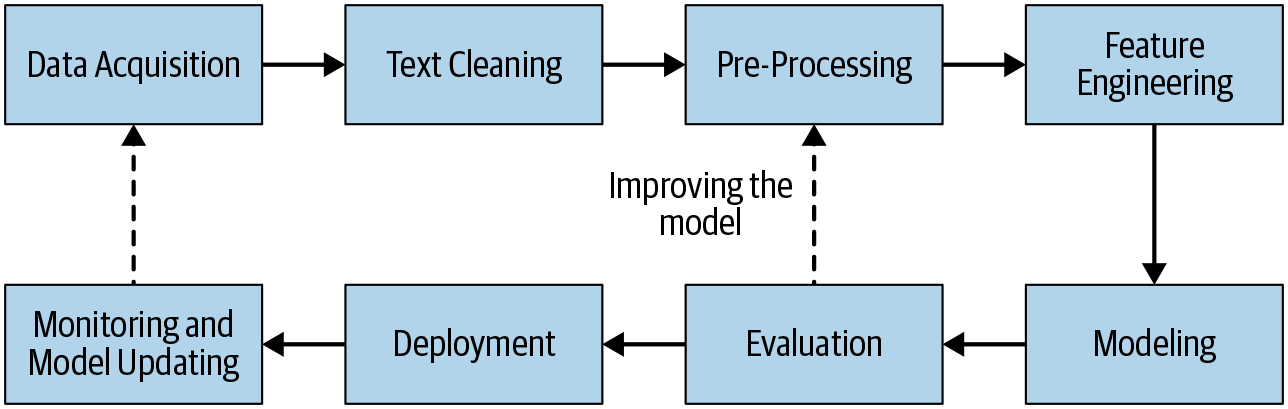
\includegraphics[width=\textwidth]{figures/pipeline.png} \pause
-the first step is "data acquisition". Why do we need it at all
\end{frame}

\begin{frame}
\frametitle{}
\Large Data Acquisition/Corpus Collection
\newline \tiny note: I am going to use corpus and data/dataset interchangeably.
\end{frame}

\begin{frame}
\frametitle{Why do we need data at all?}
my one line answer: to teach the machine! \pause
\begin{itemize}
\item Modern NLP is heavily machine learning driven and machine learning approaches typically require lots and lots of examples to "train" on and learn a task. \pause
\item Assuming we are "engineering" everything manually, we still need some kind of curated data to evaluate our approach for its accuracy and coverage.
\end{itemize}
\pause So, good quality datasets are very (very) important for building any NLP system. 
\end{frame}

\begin{frame}
\frametitle{Why collect our own data?}
\begin{itemize}
\item Clearly, building and evaluating NLP systems requires some corpus or the other.
\item When we are working on developing new methods/algorithms, we often work with standard/pre-existing datasets to compare among different approaches. \pause
\item However, when we are working on using NLP for a specific problem scenario, we won't often have such datasets that meet our exact needs.
\item Data can come in various forms, but in most cases, we need some form of "labeled" data. (What's that?)
\end{itemize}
\end{frame}

\begin{frame}
\frametitle{What kind of data do we need for NLP? -1}
\begin{itemize}
\item Huge collections of text (language modeling, topic modeling etc)  \pause 
\item Lot of examples of expected input $->$ expected output pairs. E.g., 
\begin{itemize}
\item sentence-translated sentence pairs (machine translation)
\item spam/non-spam emails (spam classification)
\item question-answer pairs
\item sentence $->$ names of entities in it, relations between them etc (information extraction)
\end{itemize}
\end{itemize}
.... 
Data can come in various forms, but in most cases, we need some form of "labeled" data (i.e., input $->$ output pairs). 
\end{frame}

\begin{frame}{What kind of data do we need? - 2}
\begin{itemize}
    \item Quantity: Typically, "learning" methods are data hungry. The more, the better, although it may plateau at some point. (What is large?) \pause
    \item Quality: Garbage in $->$ Garbage out. We can't take \textbf{anything} we can lay hands on. (Why?) \pause
    \item Data without ethical concerns such as using data without consent, keeping personally identifiable information, racial/gender bias in training examples etc. (Why is this important?) \pause
    \item (Ideally) Variety: spoken language, social media, literary texts, dialect variation, legal docs, non-native language, different topics/subjects etc (Why?) 
\end{itemize}
\end{frame}

\begin{frame}
\frametitle{How do we collect a corpus?}
\framesubtitle{1. Use available data}
There are many openly (most of them are free) accessible NLP datasets. 
\begin{itemize}
    \item \href{https://datasets.quantumstat.com/}{Quantum Stats NLP database}
    \item \href{https://huggingface.co/datasets}{Hugging Face NLP datasets}
    \item \href{https://www.ldc.upenn.edu/}{Linguistic Data Consortium}
    \item Researchers and organizations sometimes release their datasets for public (check research papers/company blog posts etc)
\end{itemize}
\end{frame}

\begin{frame}{An Exercise}
In the breakout rooms: spend 15 minutes and look for publicly available datasets in any two languages (first language: English or German, second language - choose something that is not widely spoken or if you don't know if NLP resources exist for that language).

Make a note on how big is this dataset, and any details (if mentioned) about what are its contents (i.e., what kind of text is it?), where is it useful etc. I will ask each room to do a 2 minute summary of their findings afterwards. 
\end{frame}

\begin{frame}{Discussion about findings}
    
\end{frame}

\begin{frame}
\frametitle{How do we collect a corpus?}
\framesubtitle{2. Collect your own data}
\begin{itemize}
\item Use existing data on the web
\begin{itemize}
\item scraping websites (forums, newspapers, wikipedia etc)
\item collecting social media content (blog posts, tweets etc)
\item newspapers, wikipedia etc. 
\item public archives (copyright free books, parliament proceedings, others)
\end{itemize}
\item Collect your own (crowd sourcing, user studies, surveys etc)
\end{itemize}
Let us see some examples for each. 
\end{frame}

\begin{frame}
\frametitle{How do we collect a corpus?}
\framesubtitle{2. Collect your own data}
Scraping websites
\begin{itemize}
    \item In a recently reported research work, researchers in USA collected a dataset of COVID-19 FAQs through webscraping (\href{https://www.aclweb.org/anthology/2020.nlpcovid19-2.31.pdf}{Process here}) \pause
    \item \href{https://www.aclweb.org/anthology/2020.lt4gov-1.3/}{This project} describes how a government body in Mexico city used web scraping and NLP for improving job search experience. 
  \pause  \item personal experiences:  While working at SfS, I and Prof. Meurers collected data for training machine learning models using several websites (Weekly Reader, BBC Bitesize, Geo-Geolino (German), Time- Time for Kids etc) \pause
    \item While working at a company long back, I collected question-answer pairs from a lot of forum websites, to build a search engine. 
\end{itemize}
\end{frame}

\begin{frame}
\frametitle{How do we collect a corpus?}
\framesubtitle{2. Collect your own data}
public archives, newspapers, Wikipedia etc
\begin{itemize}
    \item Parliament proceedings from European Parliament (EUROPARL - several languages), Hansard in Canada (English-French), Nunavut Hansard (English-Inuktitut) etc. are commonly used as training corpora for machine translation.
    \item Crawled and annotated corpora from WSJ, NYT etc are frequently used as training data in NLP (you may have noticed if you browsed LDC). \pause
\pause    \item personal experiences:  While working at a company, I scraped Canadian supreme court websites for case summaries. \pause
\item I also crawled Wikipedia to build a labeled dataset of various categories of articles related to legal domain (e.g., finance law, human rights law etc) to develop a document tagger.
\end{itemize}
\end{frame}

\begin{frame}
\frametitle{How do we collect a corpus?}
\framesubtitle{2. Collect your own data}
Social media content
\begin{itemize}
    \item Twitter is a common source of data to study various issues such as trending topics, fake news, offensive text detection, sentiment analysis etc.
    \item It is also useful in industry scenarios for customer support, product reviews etc.
    \item Other social media websites such as Facebook, Reddit etc are also regularly used to collect data in NLP. 
    \item \href{https://www.aclweb.org/anthology/search/?q=twitter}{This link} shows how common it is to use such data for NLP Research!
\end{itemize}
\end{frame}

\begin{frame}
\frametitle{How do we collect a corpus?}
\framesubtitle{2. Collect your own data}
crowd sourcing, user studies etc
\begin{itemize}
    \item Crowdsourced datasets from \href{Microsoft}{https://msropendata.com/datasets?term=crowdsourcing} and other such large organizations (Google etc) \pause
    \item Crowdsourcing for compamy's internal use: Google collects \href{https://translate.google.com/contribute}{translation data} through user contributions
    \pause \item personal experiences:  In 2016, Prof Meurers and I collected eye-tracking experiment data to study an NLP problem, by collaborating with cognitve science researchers at IWM-Tuebingen. 
    \item in 2018, I and my student \href{https://github.com/nishkalavallabhi/BEA19UserstudyData}{collected data} through a user study where university students read texts and answered questions about them. \pause
    \item Our own data can also come from internal organizational data sources like search logs, customer support data etc. 
\end{itemize}
\end{frame}

\begin{frame}
\frametitle{How do we collect a corpus?}
\framesubtitle{"Annotated" Data?}
\begin{itemize}
    \item In some of these examples (scraping q\&a, crawling Wikipedia with categories), we see data that does not need additional annotations. \pause
    \item In others, we wonder where the labels (e.g., positive vs negative sentiments, fake news vs normal), where does the labeled/annotated data come from? \pause
    \item crowd sourcing or having a more structured annotation experiments are two common ways of getting them.
\end{itemize}
%complete the slide
\end{frame}

\begin{frame}
\frametitle{How do we collect a corpus?}
\framesubtitle{Active Learning}
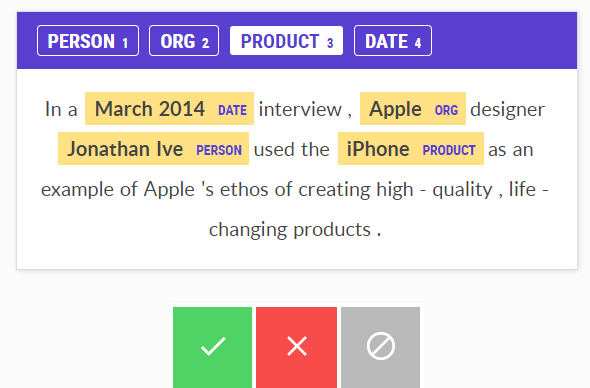
\includegraphics[width=\textwidth]{figures/prodigy.png}

\tiny \href{https://prodi.gy/}{Source}

(I briefly talked about this in the last class)
\end{frame}


\begin{frame}{Annotation Tools}
\begin{itemize}
    \item Several tools exist, each serving its own purpose. 
    \item Recent, open-source tool of interest, especially for small projects: \href{https://github.com/doccano/doccano}{Doccano}
    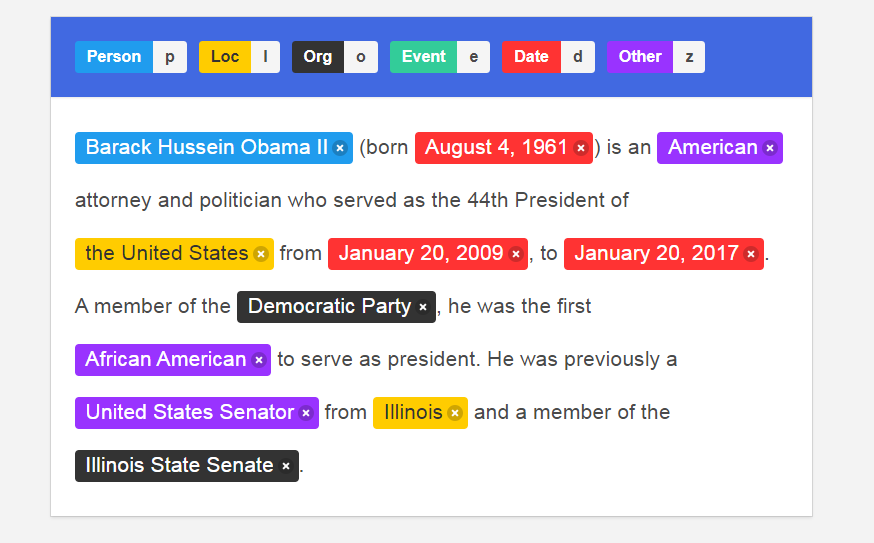
\includegraphics[width=\textwidth]{figures/Doccano.PNG}
\end{itemize}
    
\end{frame}

\begin{frame}{An Exercise}
In the breakout rooms (15 minutes): go to https://datasets.quantumstat.com/ and look for datasets collected using various ways we just saw. You don't have to cover each and every possibility - just be ready to discuss about say 3 datasets collected from different sources (i.e., one from social media, one from crowd sourcing, one from news/wiki,), and comment on how big they are, what language they are in etc.

Each group should summarize their findings after 15 minutes. 
\end{frame}

\begin{frame}{An Exercise}
Summary of your breakout room discussions.
\end{frame}

\begin{frame}[fragile]
\frametitle{How do we collect a corpus?}
\framesubtitle{3. "Generate" your own data}
\begin{itemize}
    \item Data labeling: Look for patterns in the data, and generate labels using string matching, regular expressions etc.
    \item Data Augmentation: Generate synthetic data to add to what is already there through various strategies like - replacing words with synonyms, back translation, replacing names etc.
    \item Active Learning: interactively labeling the text to teach the learning algorithm 
\end{itemize}
\end{frame}

\begin{frame}[fragile]
\frametitle{How do we collect a corpus?}
\framesubtitle{3. "Generate" your own data}
Data Labeling
\begin{itemize}
\item e.g., using labeling functions in Snorkel: noisy, programmatic rules and heuristics that assign labels to unlabeled training data. 
    \tiny
    \begin{verbatim}
from snorkel.labeling import labeling_function

@labeling_function()
def lf_contains_link(x):
    # Return a label of SPAM if "http" in comment text, otherwise ABSTAIN
    return SPAM if "http" in x.text.lower() else ABSTAIN

@labeling_function()
def check_out(x):
    return SPAM if "check out" in x.text.lower() else ABSTAIN

\end{verbatim}
\end{itemize}
More at: \url{https://www.snorkel.org/use-cases/} \\ (Topic for next class)
\end{frame}

\begin{frame}
\frametitle{How do we collect a corpus?}
\framesubtitle{3. "Generate" your own data}
Data Augmentation: Replacing words with synonyms (of different kinds) 

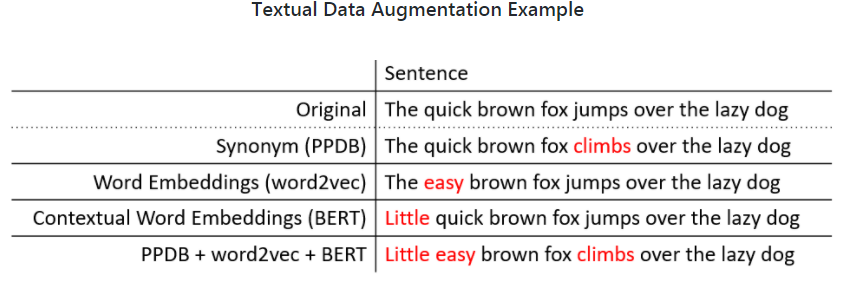
\includegraphics[width=\textwidth]{figures/augmentation1.PNG}

\tiny \href{https://github.com/makcedward/nlpaug}{source}
\end{frame}

\begin{frame}
\frametitle{How do we collect a corpus?}
\framesubtitle{3. "Generate" your own data}
Data Augmentation: Back Translation

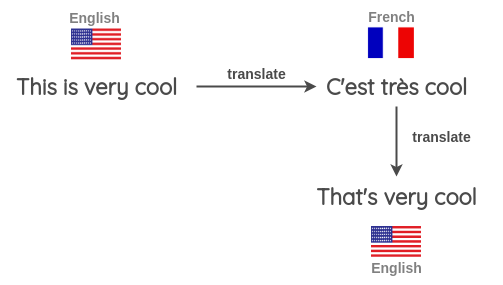
\includegraphics[width=\textwidth]{figures/backtranslation.PNG}

\tiny \href{https://amitness.com/2020/05/data-augmentation-for-nlp/}{Source}

(more on this on Monday)
\end{frame}


\begin{frame}{A fun Exercise}
In the breakout rooms (10 minutes): Try some back translation using Google or Bing translate (i.e., type a sentence in one language to translate to another. Now, take the translated sentence, translate it back to original language). Share your observations after trying a few examples. Did you notice something interesting? Something funny? How can this be a useful data collection method according to you? Each group should summarize their findings after 10 minutes. 
\end{frame}


\begin{frame}{}
Summary of your breakout room discussions.
\end{frame}

\begin{frame}{Different Ways of acquiring data: a summary}
    \begin{itemize}
        \item Using existing public datasets
        \item Scraping data from websites, social media, public archives etc.
        \item Collecting our own data (crowd sourcing, user studies etc), setting up annotation experiments, Active learning etc
        \item Data Labeling
        \item Data augmentation
    \end{itemize}
\end{frame}

\begin{frame}{Some practical issues with data collection}
        %gratis-libre paper summary? 
\begin{itemize}
    \item Clearly, there are benefits with scraping data from websites of various kinds.
    \item What are some potential risks? \pause
    \begin{enumerate}
        \item user created, publicly available data can pose privacy risks for individuals who created it. \pause (sometimes, datasets are released after anonymization).
        \item you may be collecting the data without asking for permissions (ask: is everything freely visible on the web essentially free for such use?)
        \item copyrights/terms of service conflicts may come up. \pause
        \item Often, websites' policies allow free browsing, but not crawling. 
    \end{enumerate}
\end{itemize}

\tiny Diesner, J., \& Chin, C. L. (2016, May). Gratis, libre, or something else? Regulations and misassumptions related to working with publicly available text data. In Actes du Workshop on Ethics In Corpus Collection, Annotation \& Application (ETHI-CA2), LREC, Portoroz, Slovénie.
\end{frame}

\begin{frame}{Datasheets for Datasets-1}
Ask the following while creating/using a dataset
\begin{enumerate}
    \item Why was the dataset created? Who funded its creation? How and when was it created?
    \item Who were involved in the collection? (students, crowdworkers etc.) How were they compensated?
    \item What preprocessing/cleaning was done?
    \item How is the dataset released/distributed? 
    \item Will the dataset be updated? How often? by whom?
\end{enumerate}
Source: \href{http://www.fatml.org/media/documents/datasheets_for_datasets.pdf}{"Datasheets for Datasets", Gebru et.al., 2018}
\end{frame}

\begin{frame}
\frametitle{Datasheets for Datasets-2}
Legal and Ethical considerations
\begin{itemize}
\item  If it relates to people, were they told what the dataset would be used for and did they consent?
\item If it relates to people, could this dataset expose people to harm or legal action?
\item If it relates to people, does it unfairly advantage or dis-advantage a particular social group?
\item Does the dataset comply with the EU General Data Protection Regulation (GDPR)?
\end{itemize}
\footnotesize
Full list of questions in the original paper linked in the previous slide. Bender \& Friedman, 2018 is another good paper on the topic of corpora creation/use (it is in our syllabus' readings section). 
\end{frame}

\begin{frame}
\frametitle{Corpus Collection: Summary}
\begin{itemize}
\item There are many ways to get data, and label it.
\item There are some concerns to be addressed while doing it too. 
\item I hope this part of today's class gave you a broad overview of all things related to data in NLP. \pause
\item Some questions:
\begin{itemize}
\item What are some sources of data for your native language? (if it is not English/German). 
\item Do you need annotated data? what sort of annotations are needed? How do you get them? - think about these questions. 
\end{itemize}
\end{itemize}
\end{frame}

\begin{frame}
\frametitle{Class Outline}
\begin{itemize}
    \item Quick recap of last class
    \item Corpus Collection
    \item \textbf{Text Extraction}
    \item Corpus Exploration
\end{itemize}
We can take a short 5 min break if you want. 
\end{frame}

\begin{frame}
\frametitle{Text Extraction - some questions}
\begin{itemize}
\item Why should we know how to work with various file formats?
\item How do we extract text from different file formats?
\item What are some problems with existing solutions?
\end{itemize}
source material: Chapter 2 from \url{https://practicalnlp.ai}
\end{frame}

\begin{frame}
\frametitle{Why different formats?}
\begin{itemize}
\item Generally, when we learn NLP, we work with existing data, already converted to plain text.
\item However, real world scenarios are far from this.
\item That said, documents can come in many different formats. We better have at least a vague idea of extracting text from those formats!
\end{itemize}
\end{frame}

\begin{frame}
\frametitle{Some example formats}
\begin{itemize}
\item PDFs
\item scanned texts/image files
\item XML files
\item HTML files such as web pages, forums etc. 
\item live Twitter stream
\item already existing tweets stored in a database/.csv file etc.
\item JSON
\item Docx files
\item Data stored in the cloud
\item **best format* txt files, other plain text files
\end{itemize}
... ...
\end{frame}

\begin{frame}
\frametitle{Reading from HTML/XML}
What we need: bs4 library in Python
\begin{itemize}
\item We have to understand the structure of the document/tags used etc (e.g., inspect element in chrome browser) to be able to extract.
\item What happens behind the scenes: The library "parses" HTML/XML formatted text and builds a tree like object of the format, so that we can query and extract what we want. 
\end{itemize}
\tiny details: \url{https://pypi.org/project/beautifulsoup4/}
\end{frame}

\begin{frame}{bs4 - an example}
    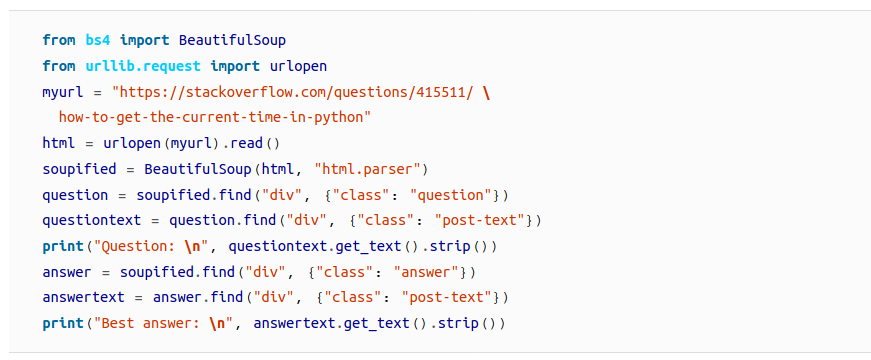
\includegraphics[width=\textwidth]{figures/bs4example.png}
    \tiny note: current version of stackoverflow does not work with this code, as they changed their layout. 
\end{frame}

\begin{frame}
\frametitle{Reading from JSON}
What we need: json library (just import json)
\begin{itemize}
\item JSON is a commonly used format to exchange data, including text.
\item Good thing with this is: it is natively supported by Python, and it looks like a lot of dictionary objects when you see. 
\item We still have to figure out the structure to get what we want. 
\end{itemize}
\tiny details: \url{https://realpython.com/python-json/}
\end{frame}

\begin{frame}
\frametitle{Reading from PDFs}
What we need: pypdf2 library is a good start. 
\begin{itemize}
\item There are many such libraries for pdf parsing, each good at a certain kind of data.
\item camelot/tabula/excalibur-py can be used to extract tabular data from pdfs.
\item Google/Amazon are now offering some tools in their web-based (paid) services.
\item Yet, I did not come across a perfect solution so far. 
\item Very challenging format to process. 
\end{itemize}
\tiny useful link: \url{https://realpython.com/pdf-python/}
\end{frame} 

\begin{frame}
\frametitle{Reading from twitter stream}
What we need: tweepy
\begin{itemize}
\item We need a twitter account, and some authentication tokens for using twitter through a program
\item This is a good source of streaming, latest data
\item However, be aware of Twitter's terms of use, don't store identifying information, and remember: many NLP tools don't work well on tweets. So, look for custom variants (they exist). 
\end{itemize}
\tiny
details: \url{https://www.earthdatascience.org/courses/use-data-open-source-python/intro-to-apis/twitter-data-in-python/}
\end{frame}

\begin{frame}[fragile]
\frametitle{Reading from scanned images}
What we need: OCR (Optical Character Recognition)
\begin{verbatim}
from PIL import Image
from pytesseract import image_to_string
filename = "somefile.png"
text = image_to_string(Image.open(filename))
print(text)
\end{verbatim}
\tiny details: \url{https://pypi.org/project/pytesseract/}
\end{frame}

\begin{frame}
\frametitle{Text Extraction: Summary}
\begin{itemize}
\item Many different file formats
\item Many different libraries for each
\item They may not be perfect - but it could meet your needs, depending on what level of NLP you want/need
\item However, some formats such as pdfs or images can never give you a perfect solution.
\item What to do with what we managed to extract?
\end{itemize}
... ...
\tiny \url{https://nostarch.com/automatestuff2} - this free ebook has a lot of code examples on extracting data from different formats. 
\end{frame}

\begin{frame}{Class Outline}
\begin{itemize}
    \item Quick recap of last class
    \item Corpus Collection
    \item Text Extraction
    \item \textbf{Corpus Exploration}
\end{itemize}
\end{frame}

\begin{frame}
\frametitle{Corpus Exploration - Goals}
\begin{itemize}
\item Understand what corpus analysis is and why it is needed
\item Do some basic analyses
\item source: Chapter 1-2 in nltk.org/book, and a few linked blog posts
\end{itemize}
\end{frame}

\begin{frame}
\frametitle{What is corpus exploration?}
\begin{itemize}
\item Understanding what's in the corpus:
\begin{itemize}
\item Looking at frequently used words/ngrams in the corpus
\item What words go together? (collocations)
\item Other properties of the corpus such as lexical diversity, linguistic coverage etc.
\item What categories are more frequent/less frequent etc. 
\end{itemize}
\item How can we visualize a corpus quickly? 
\end{itemize}
.. ... 
\end{frame}

\begin{frame}
\frametitle{Why? }
\begin{itemize}
\item Understand what the texts are about (generally speaking)
\item What can be some useful features to use in an NLP model for this corpus
\item Identify potential noise in the data  
\item Understand the limitations (may be something you want is not represented in the corpus? may be the data is heavily unbalanced and only some kinds of text are over represented?)
\end{itemize}
\end{frame}

\begin{frame}{How?}
\framesubtitle{Some basic analyses}
    \begin{itemize}
        \item Length of documents, average sentence length etc.
        \item Specific measure such as lexical diversity etc may be useful in some cases.
        \item For text classification, for example, it is useful to look at the distribution of various categories in the corpus, most common words per category etc.
    \end{itemize}
\end{frame}

\begin{frame}[fragile]
\frametitle{On the entire corpus}
I am taking the example texts that come with nltk in this example: 
\tiny
\begin{verbatim}
from nltk.book import * #loads some sample texts
texts() #lists the texts.
list(text1) #shows a text as a list of words.

largercorpus = Text(list(text1) + list(text2) + list(text3))
\end{verbatim}

What we can do with this corpus:
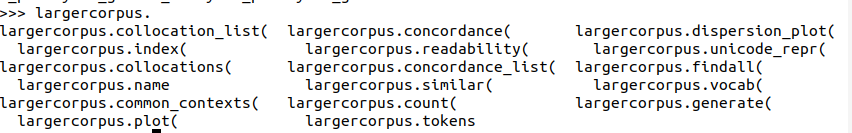
\includegraphics[width=0.9\textwidth]{figures/largercorpus.png}

\end{frame}

\begin{frame}[fragile]
\frametitle{Frequency Distributions}
\begin{verbatim}
fdist = FreqDist(largercorpus)
\end{verbatim}

What we can do with this fdist object:
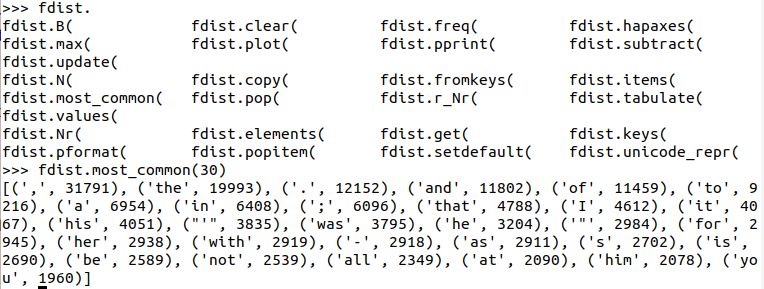
\includegraphics[width=0.9\textwidth]{figures/fdist.png}

\end{frame}

\begin{frame}[fragile]
\frametitle{How? - Frequency Distributions of ngrams}
\tiny
\begin{verbatim}
from collections import Counter
from nltk import ngrams
ngram_counts = Counter(ngrams(largercorpus, 4)) #4 for bigrams, 3 for trigrams ...
ngram_counts.most_common(10)
\end{verbatim}

What we can do with this fdist object:
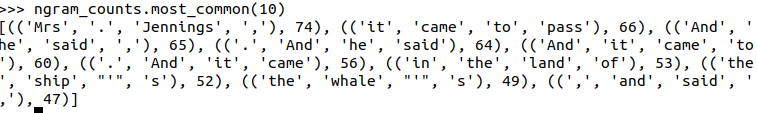
\includegraphics[width=0.9\textwidth]{figures/ngramcounts.png}
\end{frame}

\begin{frame}[fragile]
\frametitle{How? - Collocations}
"A collocation is a sequence of words that occur together unusually often. Thus red wine is a collocation, whereas the wine is not. A characteristic of collocations is that they are resistant to substitution with words that have similar senses; for example, maroon wine sounds definitely odd." 
\begin{verbatim}
largercorpus.collocation_list()
\end{verbatim}

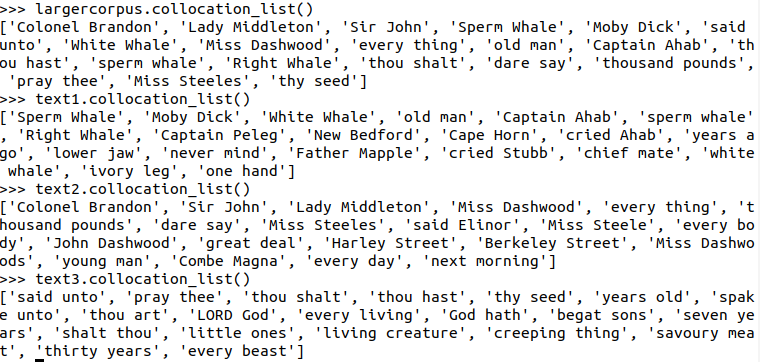
\includegraphics[width=0.9\textwidth]{figures/collocations.png}

\end{frame}

\begin{frame}{Know your pre-processing}
\begin{itemize}
\item If I am using a bag of words approach for feature engineering, what exactly are the features that are extracted? (cv.get\_feature\_names())
\item What are the stopwords I am eliminating when I import a stopword list from nltk/sklearn etc.?
\item How does my text look like after doing these pre-processing steps?
\end{itemize}
etc... \\
\tiny useful link: \url{https://kavita-ganesan.com/how-to-use-countvectorizer/}
\end{frame}

%https://medium.com/analytics-vidhya/how-to-begin-performing-eda-on-nlp-ffdef92bedf6
%https://towardsdatascience.com/nlp-part-3-exploratory-data-analysis-of-text-data-1caa8ab3f79d
%https://www.kaggle.com/wil2210/eda-nlp-ml
%https://neptune.ai/blog/exploratory-data-analysis-natural-language-processing-tools

\begin{frame}
\frametitle{Concluding Remarks on Corpus Analysis}
\begin{itemize}
\item How to make these more useful/meaningful? 
\begin{itemize}
\item Do some corpus pre-processing (e.g., lowecaser, remove stop words, punctuation etc)
\item Explore other plotting functions like wordcloud, disperson plots etc to understand data. 
\end{itemize}
\item useful tutorials: \href{https://www.kaggle.com/wil2210/eda-nlp-ml}{on Kaggle} and \href{https://neptune.ai/blog/exploratory-data-analysis-natural-language-processing-tools}{neptune.ai}
\end{itemize}
Note: Go through the first 2 chapters of the NLTK book. It has good examples of doing such exploratory analysis of a corpus. 
\end{frame}

\begin{frame}
\frametitle{Another Exercise}
Time 20 minutes, in breakout rooms.

Go to Linguistic Data Consortium's Top-10 most distributed NLP corpora (https://catalog.ldc.upenn.edu/topten). Pick any corpus you want. See if you can build a datasheet for this dataset (Look at the full list of questions at the end of Gebru et.al. 2018 paper). 

One person per team will summarize their observations at the end. Don't do exhaustively, do what you can easily understand from available material. 
\end{frame}

\begin{frame}{Next Class}
    \begin{itemize}
    \item Topic: Data Labeling, using Snorkel
    \item To Do for you: 
    \begin{enumerate}
        \item Decide on a team for group discussion (13th Jan 2021 - today!)
       \item Decide on a paper for group discussion (15th Jan 2021)
      \end{enumerate}
      \item Remember: You can email me for a meeting or post your questions in the forum for today's session "Data Collection".
    \end{itemize}
\end{frame}

\end{document}
